
\begin{figure}[t]
    \centering
    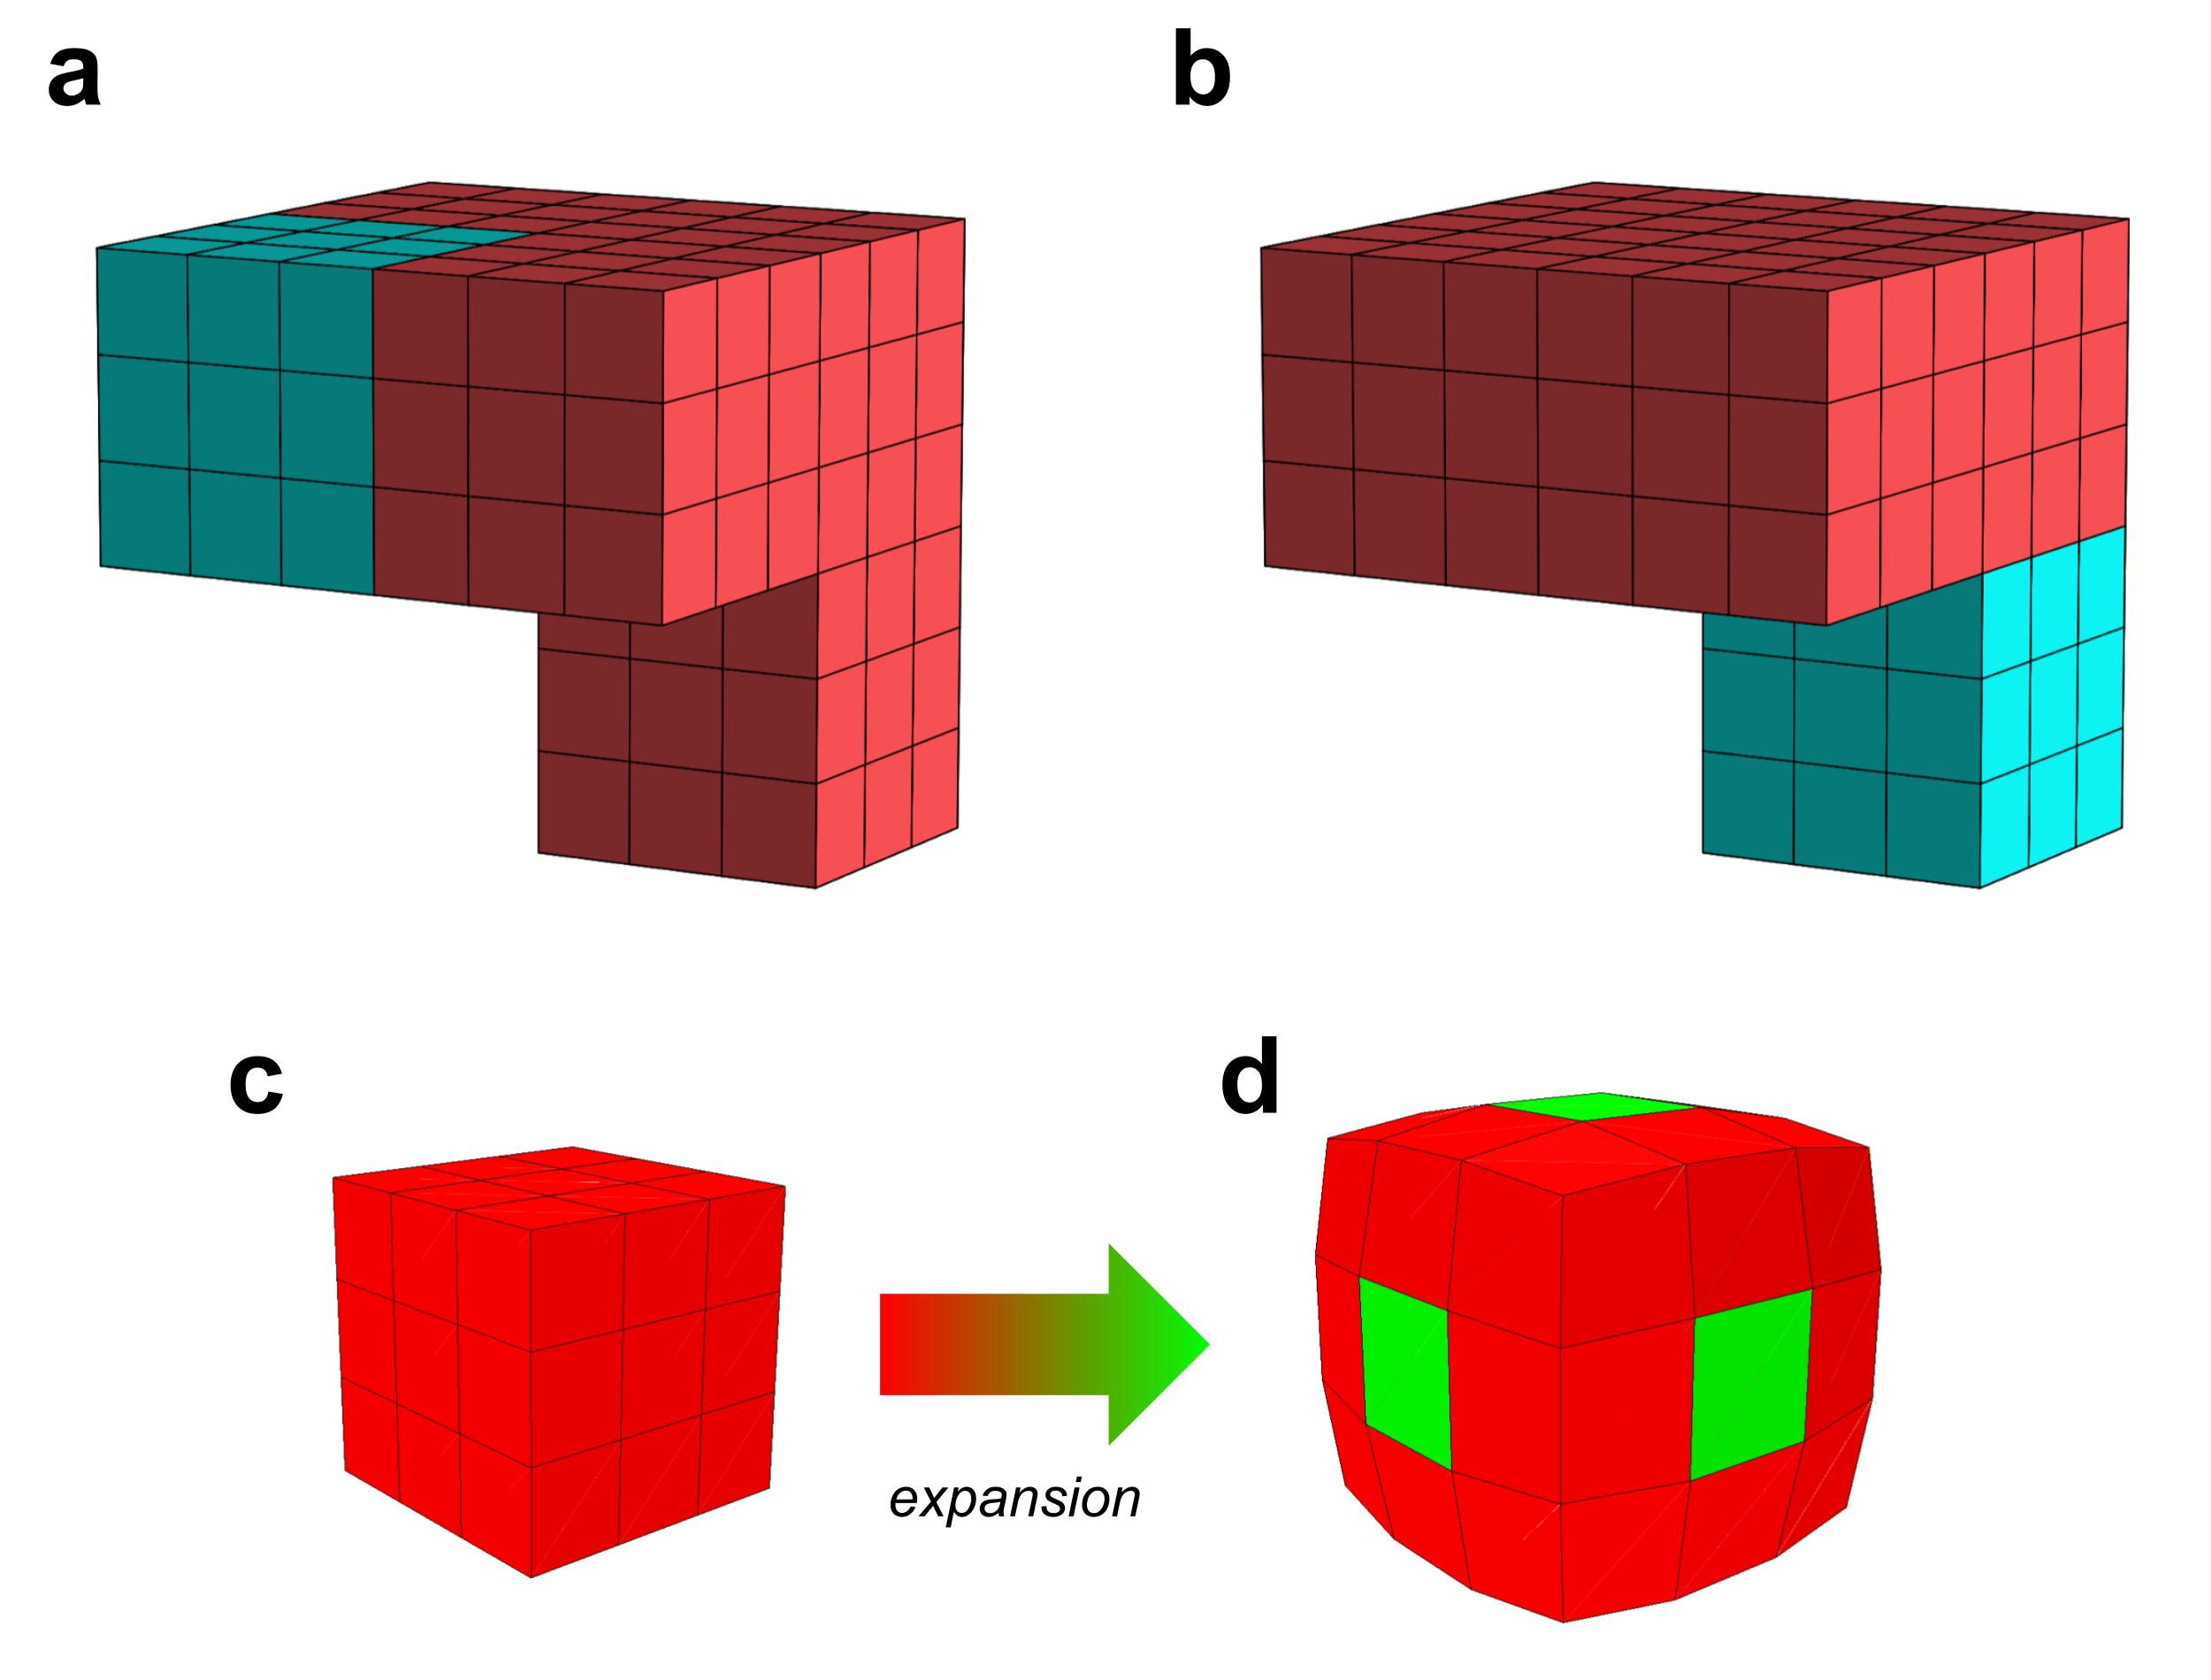
\includegraphics[width=0.65\linewidth]{Chapter02/fig/Yale_High_Res_Sim.jpg}
    % \vspace{-1em}
    \caption{A higher resolution model in which each silicone voxel is approximated by a 3-by-3-by-3 group of simulated subvoxels: a high-res voxel.
    The design in \textbf{a} and \textbf{b} are high-res instantiations of those in Figs.~\ref{fig:transfer}e and \ref{fig:transfer}f, respectively. 
    Spherical volumetric expansion in a high-res voxel (\textbf{c}) was approximated by increasing the rest length between the centermost subvoxel and the subvoxels at center of each face (green subvoxels in \textbf{d}).
    }
    \label{fig:hi_res_sim}
    % \vspace{-1.25em}
\end{figure}
